% FACULTAD DE INGENIERÍA, UNIVERSIDAD DE BUENOS AIRES
%
% 75.10 - Técnicas de Diseño
% Trabajo práctico nro 2
%
% INFORME

\documentclass[12pt]{article}

\usepackage[a4paper,headheight=16pt,scale={0.7,0.8},hoffset=0.5cm]{geometry}
\usepackage[spanish]{babel}
\usepackage{graphicx}
\usepackage[utf8]{inputenc}

% Para poner el texto "Figura X" en negrita:
\usepackage[hang,bf]{caption}

% Símbolos varios.
\usepackage{textcomp}

\title{Técnicas de Diseño: TP2}
\author{Barrios, Federico; Bosch, Florencia; Navarro, Patricio}

%------------------------- Inicio del documento ---------------------------
\begin{document}

\begin{center}
\vspace*{7 cm}
\textsc{\LARGE Universidad de Buenos Aires}\\[0.3cm]
\textsc{\LARGE Facultad de Ingeniería}\\[1.2cm]
\textsc{\Large 75.10 -- Técnicas de Diseño}\\[0.3cm]
\textsc{\Large Trabajo Práctico 2}\\[1.2cm]
\end{center}

\begin{flushright}
{\large
Grupo 3:\\[0.1cm]
Barrios, Federico -- 91954\\
Bosch, Florencia -- 91867\\
Navarro, Patricio -- 90007\\[0.4cm]
$2^{do}$ cuatrimestre de 2013}
\end{flushright}

\thispagestyle{empty}

\newpage

% Pongo el índice en una página aparte:
\tableofcontents
% Hago que las páginas se comiencen a contar a partir de aquí:
\setcounter{page}{1}
\newpage

\section{Especificación}
Se propone en esta instancia seguir agregando funcionalidades al framework de testing implementado,
con la diferencia de que esta vez desarrollamos sobre el trabajo de otro grupo. 

Los requerimientos 
pedidos por la cátedra son ahora un límite de tiempo de corrida, de manera de registrar como fallos
casos de prueba cuya ejecución exceda un tiempo dado. Además se pide una función de \textit{memoria}
para recordar aquéllos casos de pruebas que hayan terminado exitosamente, para así ejecutar en una
corrida posterior los fallados, los que devienen en error y los que se agregan. Es necesario ofrecer
dos tipos de \textit{Store}, y preferentemente una manera sencilla para que el usuario pueda agregar más.

\section{Análisis de la implementación del grupo 2}
Antes de empezar con la implementación de las funcionalidades nuevas, el grupo se propuso entender el 
funcionamiento del framework.

\subsection{Problemas encontrados}
Se identificaron los siguientes problemas:

\begin{itemize}
	\item \textbf{Código con errores:} pudimos identificar varios errores en el trabajo que tuvimos que
		corregir antes de empezar a implementar:
		
		\begin{itemize}
			\item El código contenía warnings referidos a un mal uso de la genericidad de Java.
			
			\item Maven no compilaba debido a la omisión de la dependendencia que incluye el paquete 
				com.sun.javaws.				
		\end{itemize}
		
		Estos dos errores fueron los primeros en ser solucionados.
		
	\item \textbf{Documentación escasa:} el código casi no contenía comentarios salvo la descripción de las
		responsabilidades de cada clase y la documentación entregada era escasa y obsoleta; 
		por ejemplo el diagrama de clases no se ajustaba al código entregado.
		
	\item \textbf{Errores funcionales:} se detectaron varias situaciones en dónde el comportamiento
		no es el esperado de un framework de testing:
		
		\begin{itemize}
			\item El contexto del fixture puede ser modificado por cada caso de prueba, acarreando las
				modificaciones y derivando en un mal funcionamiento del resto de los tests.
				El comportamiento esperado era que el contexto no fuese modificado y que el
				resultado de la corrida sea independiente del orden de ejecución de los tests.

			\item También relacionado con lo anterior, el contexto no permitía almacenar objetos de cualquier 
				tipo, que es lo esperado de un framework.
				
			\item El resultado de la corrida en formato XML no respeta el esquema modelo brindado por 
				el curso.
				
			\item Las corridas de cada test figuraban con un tiempo de ejecución diferente en cada
				tipo de reporte. Esto se debía a que se detenía el temporizador en la función de
				escritura.

		\end{itemize}	
		
	\item \textbf{Violación de los principios de diseño:} nos resultó muy complicada la tarea de implementar 
		las funcionalidades nuevas debido a que el diseño no respetaba el principio de clausura ante 
		cambios y apertura ante modificaciones; imposibilitando, incluso, la adición de ciertas pruebas. 
		Además, la clase TestReport tiene muchas responsabilidades.	

	\item \textbf{Uso de herramientas tecnológicas:} en la clase TestSuite, a la hora de exportar
		el reporte se usa reflexión para diferenciar el tipo del Test pasado por parámetro,
		pudiendo ser alguna de las dos clases que heredan de ella: TestCase o TestSuite.
		Vemos esto como una violación grave del paradigma de orientación a objetos y de la
		consigna del enunciado.
	
	\item \textbf{Poca cantidad de pruebas:} notamos que el trabajo tiene muy pocas pruebas
		implementadas, resultando dificultosa la tarea de añadir funcionalidades y
		de refactorizar, dado que no podemos asegurar el funcionamiento correcto del trabajo
		después de haber modificado o agregado código.
		
	\item \textbf{Estilo:} muchas variables no respetan la convención \textit{camelCase} 
		de Java; además, el estilo de ubicación de llaves y demás no es coherente dentro del
		código.
		
\end{itemize}


\section{Diseño}
Se refactorizó parte del código para que sea más sencillo implementar las funcionalidades nuevas,
permitiendo, además, que el trabajo no esté tan cerrado ante cambios.

La clase TestReport, que antes tenía varias responsabilidades, ahora está dividida en TestConditions
que sirve para determinar si un test debe ser corrido o no.

Se muestra en la figura 1 un diagrama de clases del trabajo.
\begin{figure}[h!]
\begin{center}
	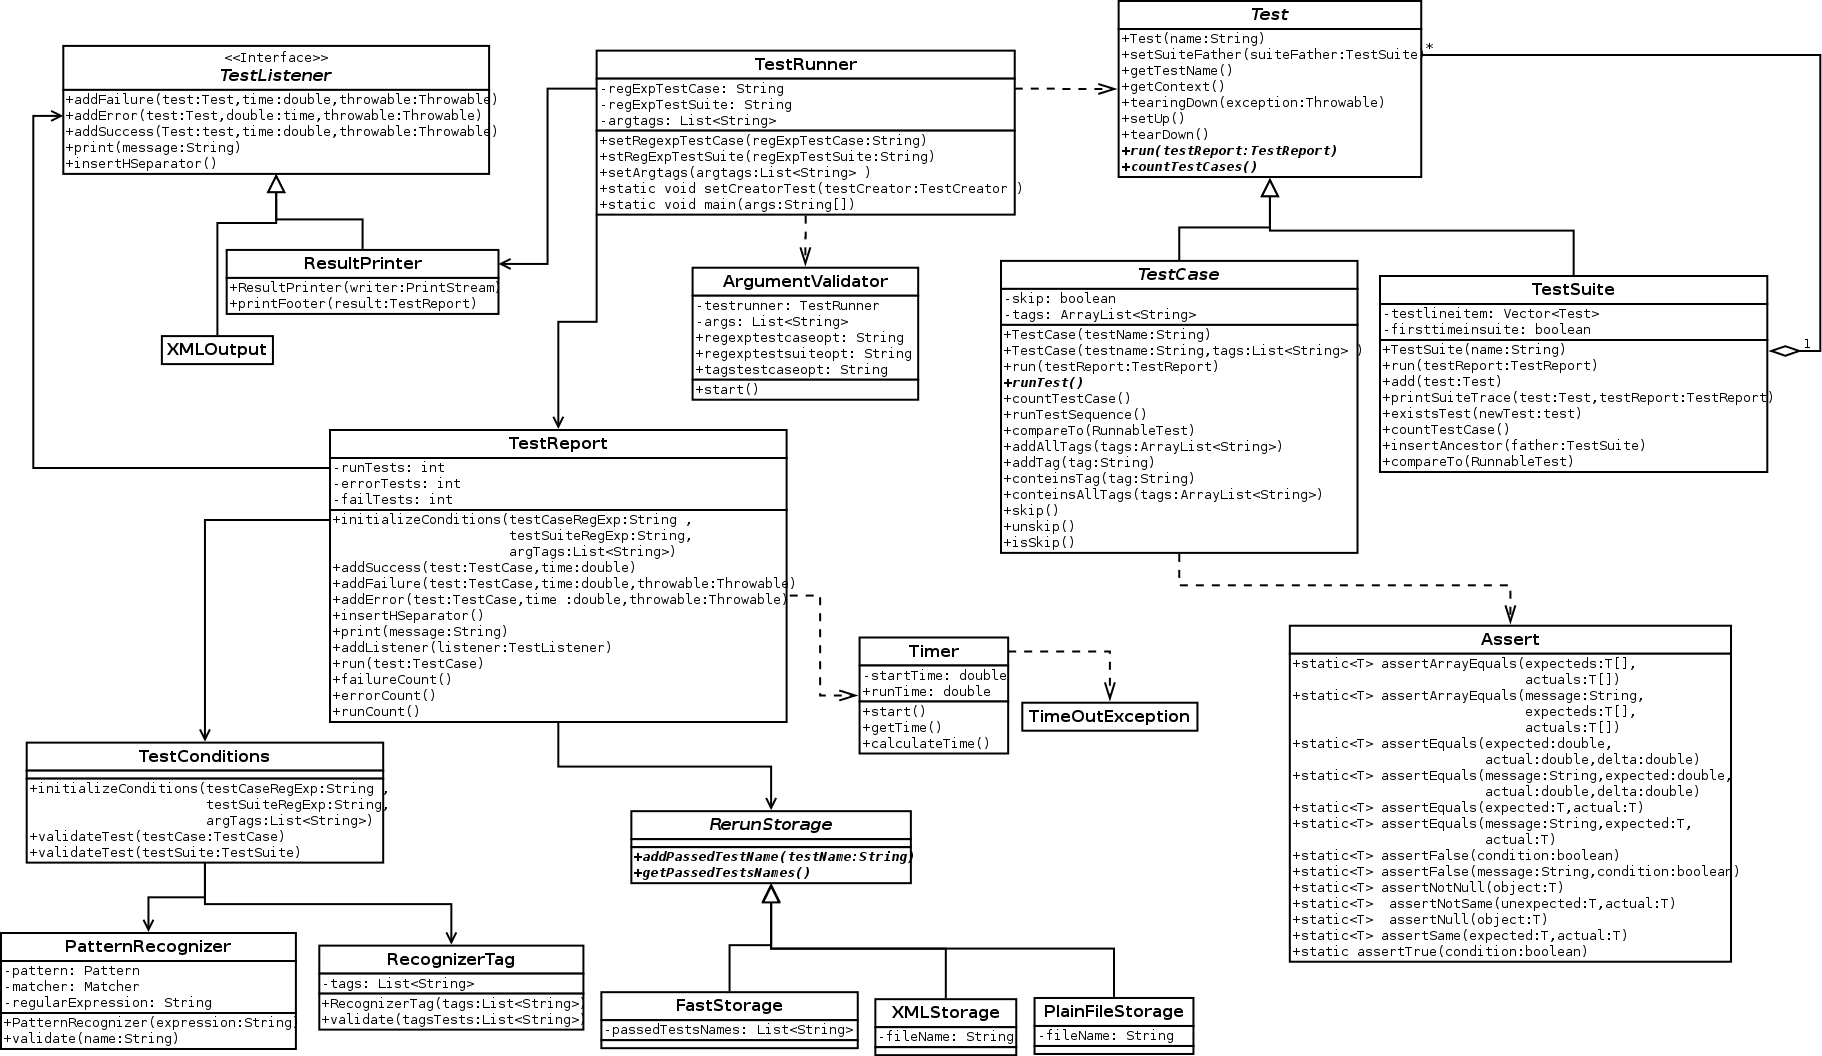
\includegraphics[scale=0.35,angle=90]{./ClassDiagram}
\end{center}
	\caption{diagrama de clases del trabajo práctico (entrega 3).}
\end{figure}

\subsection{Storage}
Esta funcionalidad fue implementada en el paquete \textit{rerunner}. Se trata de una clase
abstracta RerunStorage que define varios métodos abstractos: para agregar tests como 
ejecutados con éxito (de manera de no volver a correrlos), y para saber si un test se debe
volver a ejecutar o no. Además, permite redefinir métodos de inicialización y fin, en caso
de que el Storage lo permita. Esta interfaz simplifica la adición de Storages nuevos.

Una clase enumeradora sirve para indicar en qué modo funcionará el framework, pudiendo ser
en modo grabación (RECORD), en modo de volver a correr (RERUN) o simplemente ignorando la
persistencia (NONE).

Se incluyen implementados tres storages: FastStorage, que no persiste, sino que almacena en
memoria; XMLStorage que persiste en un archivo XML y PlainFileStorage que persiste en un
archivo de texto plano.

\subsection{Restricción temporal}
La funcionalidad de timeout se implementó añadiendo un atributo de clase a Timer, que establece
el tiempo máximo que puede tardar un caso de prueba, lanzando una excepción propia (TimeoutException) 
cuando se viola. 
Este atributo puede ser establecido por el cliente.

\subsection{Pruebas}
Se agregó el primer test unitario del framework en jUnit, llamado FrameworkTest, que contiene
las funcionalidades implementadas por el grupo; además de casos de prueba usando el mismo framework.

\section{Conclusiones}
Durante el desarrollo del trabajo práctico nos tuvimos que enfrentar con
código no escrito por nosotros, notando la importancia de algunos conceptos desarrollados
en la materia.

Por ejemplo, la falta de pruebas unitarias implicó que tuvimos que perder mucho tiempo 
simulando situaciones dado que no podíamos asegurar que nuestras modificaciones no afectaran
comportamiento antiguo. 

El diseño estaba muy cerrado ante extensiones, significando que sea necesario refactorizar 
previo a introducir funcionalidades. Tampoco contábamos con ningún tipo de documentación que nos 
ayudase a entender el código.

Concluimos en la utilidad de los conceptos que se dan en la teórica para producir software 
fácil de mantener.
\end{document}
